%versi 3 (18-12-2016)
\chapter{Kode Program}
\label{lamp:A}

%terdapat 2 cara untuk memasukkan kode program
% 1. menggunakan perintah \lstinputlisting (kode program ditempatkan di folder yang sama dengan file ini)
% 2. menggunakan environment lstlisting (kode program dituliskan di dalam file ini)
% Perhatikan contoh yang diberikan!!
%
% untuk keduanya, ada parameter yang harus diisi:
% - language: bahasa dari kode program (pilihan: Java, C, C++, PHP, Matlab, C#, HTML, R, Python, SQL, dll)
% - caption: nama file dari kode program yang akan ditampilkan di dokumen akhir
%
% Perhatian: Abaikan warning tentang textasteriskcentered!!
%


%\begin{lstlisting}[language=Java, caption=MyCode.c]
%
%// This does not make algorithmic sense, 
%// but it shows off significant programming characters.
%
%#include<stdio.h>
%
%void myFunction( int input, float* output ) {
%	switch ( array[i] ) {
%		case 1: // This is silly code
%			if ( a >= 0 || b <= 3 && c != x )
%				*output += 0.005 + 20050;
%			char = 'g';
%			b = 2^n + ~right_size - leftSize * MAX_SIZE;
%			c = (--aaa + &daa) / (bbb++ - ccc % 2 );
%			strcpy(a,"hello $@?"); 
%	}
%	count = ~mask | 0x00FF00AA;
%}
%
%// Fonts for Displaying Program Code in LATEX
%// Adrian P. Robson, nepsweb.co.uk
%// 8 October 2012
%// http://nepsweb.co.uk/docs/progfonts.pdf
%
%\end{lstlisting}

\lstinputlisting[language=Java, caption=OperasiMatematikaInterface.java]{./Lampiran/OperasiMatematikaInterface.java}
\lstinputlisting[language=Java, caption=Pembagian.java]{./Lampiran/Pembagian.java}
\lstinputlisting[language=Java, caption=Pengurangan.java]{./Lampiran/Pengurangan.java}
\lstinputlisting[language=Java, caption=Perkalian.java]{./Lampiran/Perkalian.java}
\lstinputlisting[language=Java, caption=Pertambahan.java]{./Lampiran/Pertambahan.java}
\lstinputlisting[language=TeX, caption=operasimatematika.tex]{./Lampiran/operasimatematika.tex}
\newgeometry{scale=1}
\thispagestyle{empty}
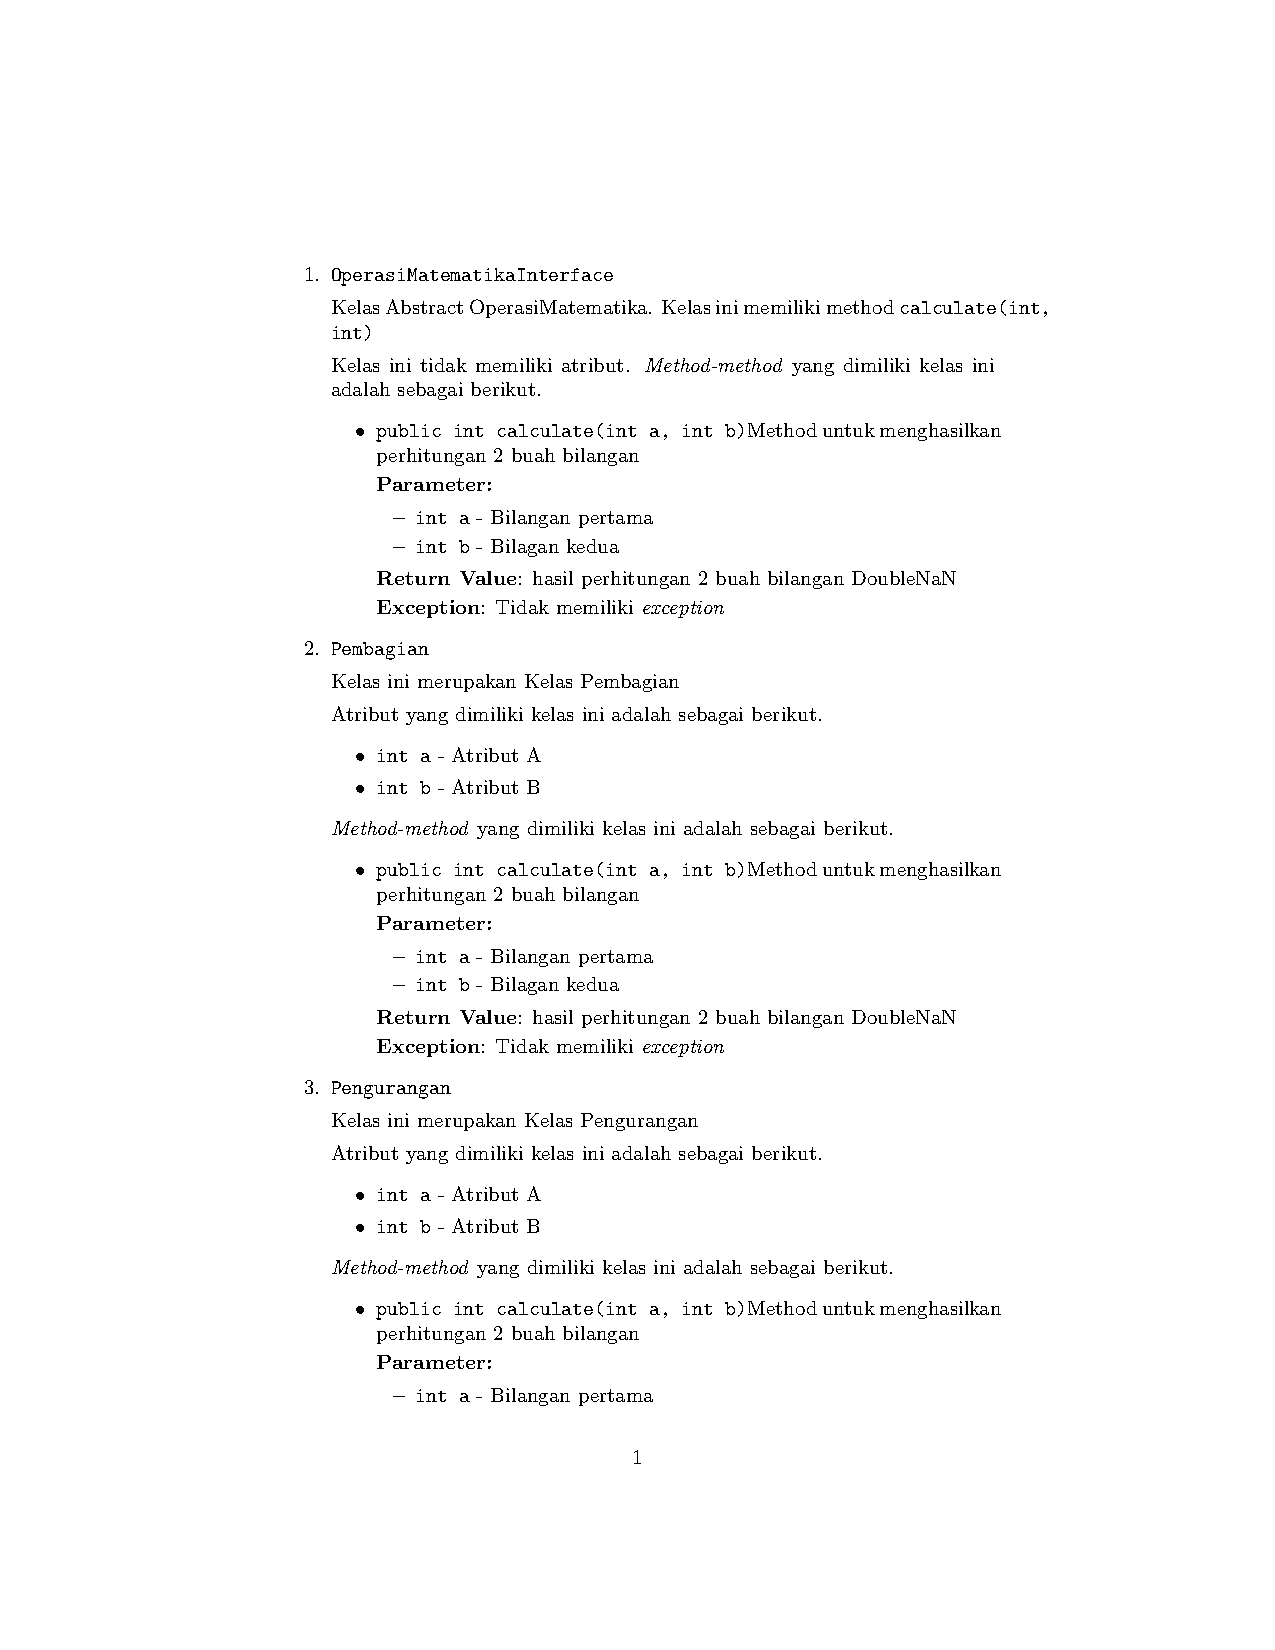
\includepdf[page=1]{./Lampiran/operasimatematika.pdf}
{
  \centering
  \includegraphics[page=2, scale=1]{./Lampiran/operasimatematika.pdf}
  \captionof{figure}{operasimatematika.pdf}
}
\restoregeometry
%\lstinputlisting[language=TeX, caption=siamodels.tex]{./Lampiran/siamodels.tex}
%\lstinputlisting[language=TeX, caption=javadoctolatex.tex]{./Lampiran/javadoctolatex.tex}

